\let\negmedspace\undefined
\let\negthickspace\undefined
\documentclass[journal]{IEEEtran}
\usepackage[a5paper, margin=10mm, onecolumn]{geometry}
%\usepackage{lmodern} 
\usepackage{tfrupee} 

\setlength{\headheight}{1cm} 
\setlength{\headsep}{0mm}     

\usepackage{gvv-book}
\usepackage{gvv}
\usepackage{cite}
\usepackage{amsmath,amssymb,amsfonts,amsthm}
\usepackage{algorithmic}
\usepackage{graphicx}
\usepackage{textcomp}
\usepackage{xcolor}
\usepackage{txfonts}
\usepackage{listings}
\usepackage{enumitem}
\usepackage{mathtools}
\usepackage{gensymb}
\usepackage{comment}
\usepackage[breaklinks=true]{hyperref}
\usepackage{tkz-euclide} 
\usepackage{listings}                                        
\def\inputGnumericTable{}                                 
\usepackage[latin1]{inputenc}                                
\usepackage{color}                                            
\usepackage{array}                                            
\usepackage{longtable}                                       
\usepackage{calc}                                             
\usepackage{multirow}                                         
\usepackage{hhline}                                           
\usepackage{ifthen}                                           
\usepackage{lscape}

\begin{document}

\bibliographystyle{IEEEtran}
\vspace{3cm}

\title{9.2.37}
\author{AI25BTECH11003 - Bhavesh Gaikwad}
{\let\newpage\relax\maketitle}

\renewcommand{\thefigure}{\theenumi}
\renewcommand{\thetable}{\theenumi}
\setlength{\intextsep}{10pt} 


\numberwithin{equation}{enumi}
\numberwithin{figure}{enumi}
\renewcommand{\thetable}{\theenumi}


\textbf{Question}: Find the area of the region bounded by the curve $x^2 = y$ and the lines $y = x + 2$ and the x-axis.

\textbf{Solution:}\\
Given: $y = x^2$ and $y = x+2$\\

The General Equation of a Conic is: 
\begin{equation}
    \vec{x}^\top\vec{V}\vec{x} + 2\vec{u}^\top\vec{x} + f = 0
\end{equation}
On comparing, we get:
\begin{equation}
    \vec{V} = \myvec{1 & 0 \\ 0 & 0}, \, \vec{u} = \myvec{0 \\ \frac{-1}{2}}, \, f =0
\end{equation}

The General Equation of a Line:
\begin{equation}
    \vec{x} = k\vec{m} + \vec{h}
\end{equation}
On comparing, we get:
\begin{equation}
    \vec{m} = \myvec{1 \\ 1}, \, \vec{h} = \myvec{0 \\ 2}
\end{equation}

The Intersection of the given conic with the given line can be written as:
\begin{equation}
    \vec{x}_i = \vec{h} + k_i\vec{m}
\end{equation}

\begin{equation}
    where, \, k_i = \left( \dfrac{1}{\vec{m}^\top\vec{V}\vec{m}} \right) \left( 
    -\vec{m}^\top(\vec{V}\vec{h}+\vec{u}) \, \pm \, \sqrt{[\vec{m}^\top(\vec{V}\vec{h}+\vec{u})]^2 - g(h)(\vec{m}^\top\vec{V}\vec{m})} \right) 
\end{equation}

Let $\vec{K} = \myvec{k_1 \\ k_2}$\\

The Solution Matrix can be expressed as: 
\begin{equation}
    \vec{X} = \myvec{\vec{h} & \vec{m}}\myvec{\vec{1} & \vec{k}}^\top
\end{equation}

Therefore, The points of intersection are:
\begin{equation}
    \vec{x}_1 = \myvec{-1 \\ 1} \quad \& \quad \vec{x}_2 = \myvec{2 \\4}
\end{equation}

\newpage

From Fig.0.1, the area bounded by the curve $y = x^2$ and line $y = x + 2$ is given by:
\begin{equation}
    \int_{-1}^{2} [(x+2) - (x^2)] \,dx = \int_{-1}^{2} [2 + x -x^2] \,dx
\end{equation}

\begin{equation}
 \int_{-1}^{2} [2 + x -x^2] \,dx = \dfrac{9}{2} = 4.5 \, sq.units   
\end{equation}

\begin{align*}
\boxed{\text{Therefore, The Area of the region bounded between $y=x^2$ and $y=x+2$ is 4.5 sq.units.}}
\end{align*}

\begin{figure}[htbp]
    \centering
    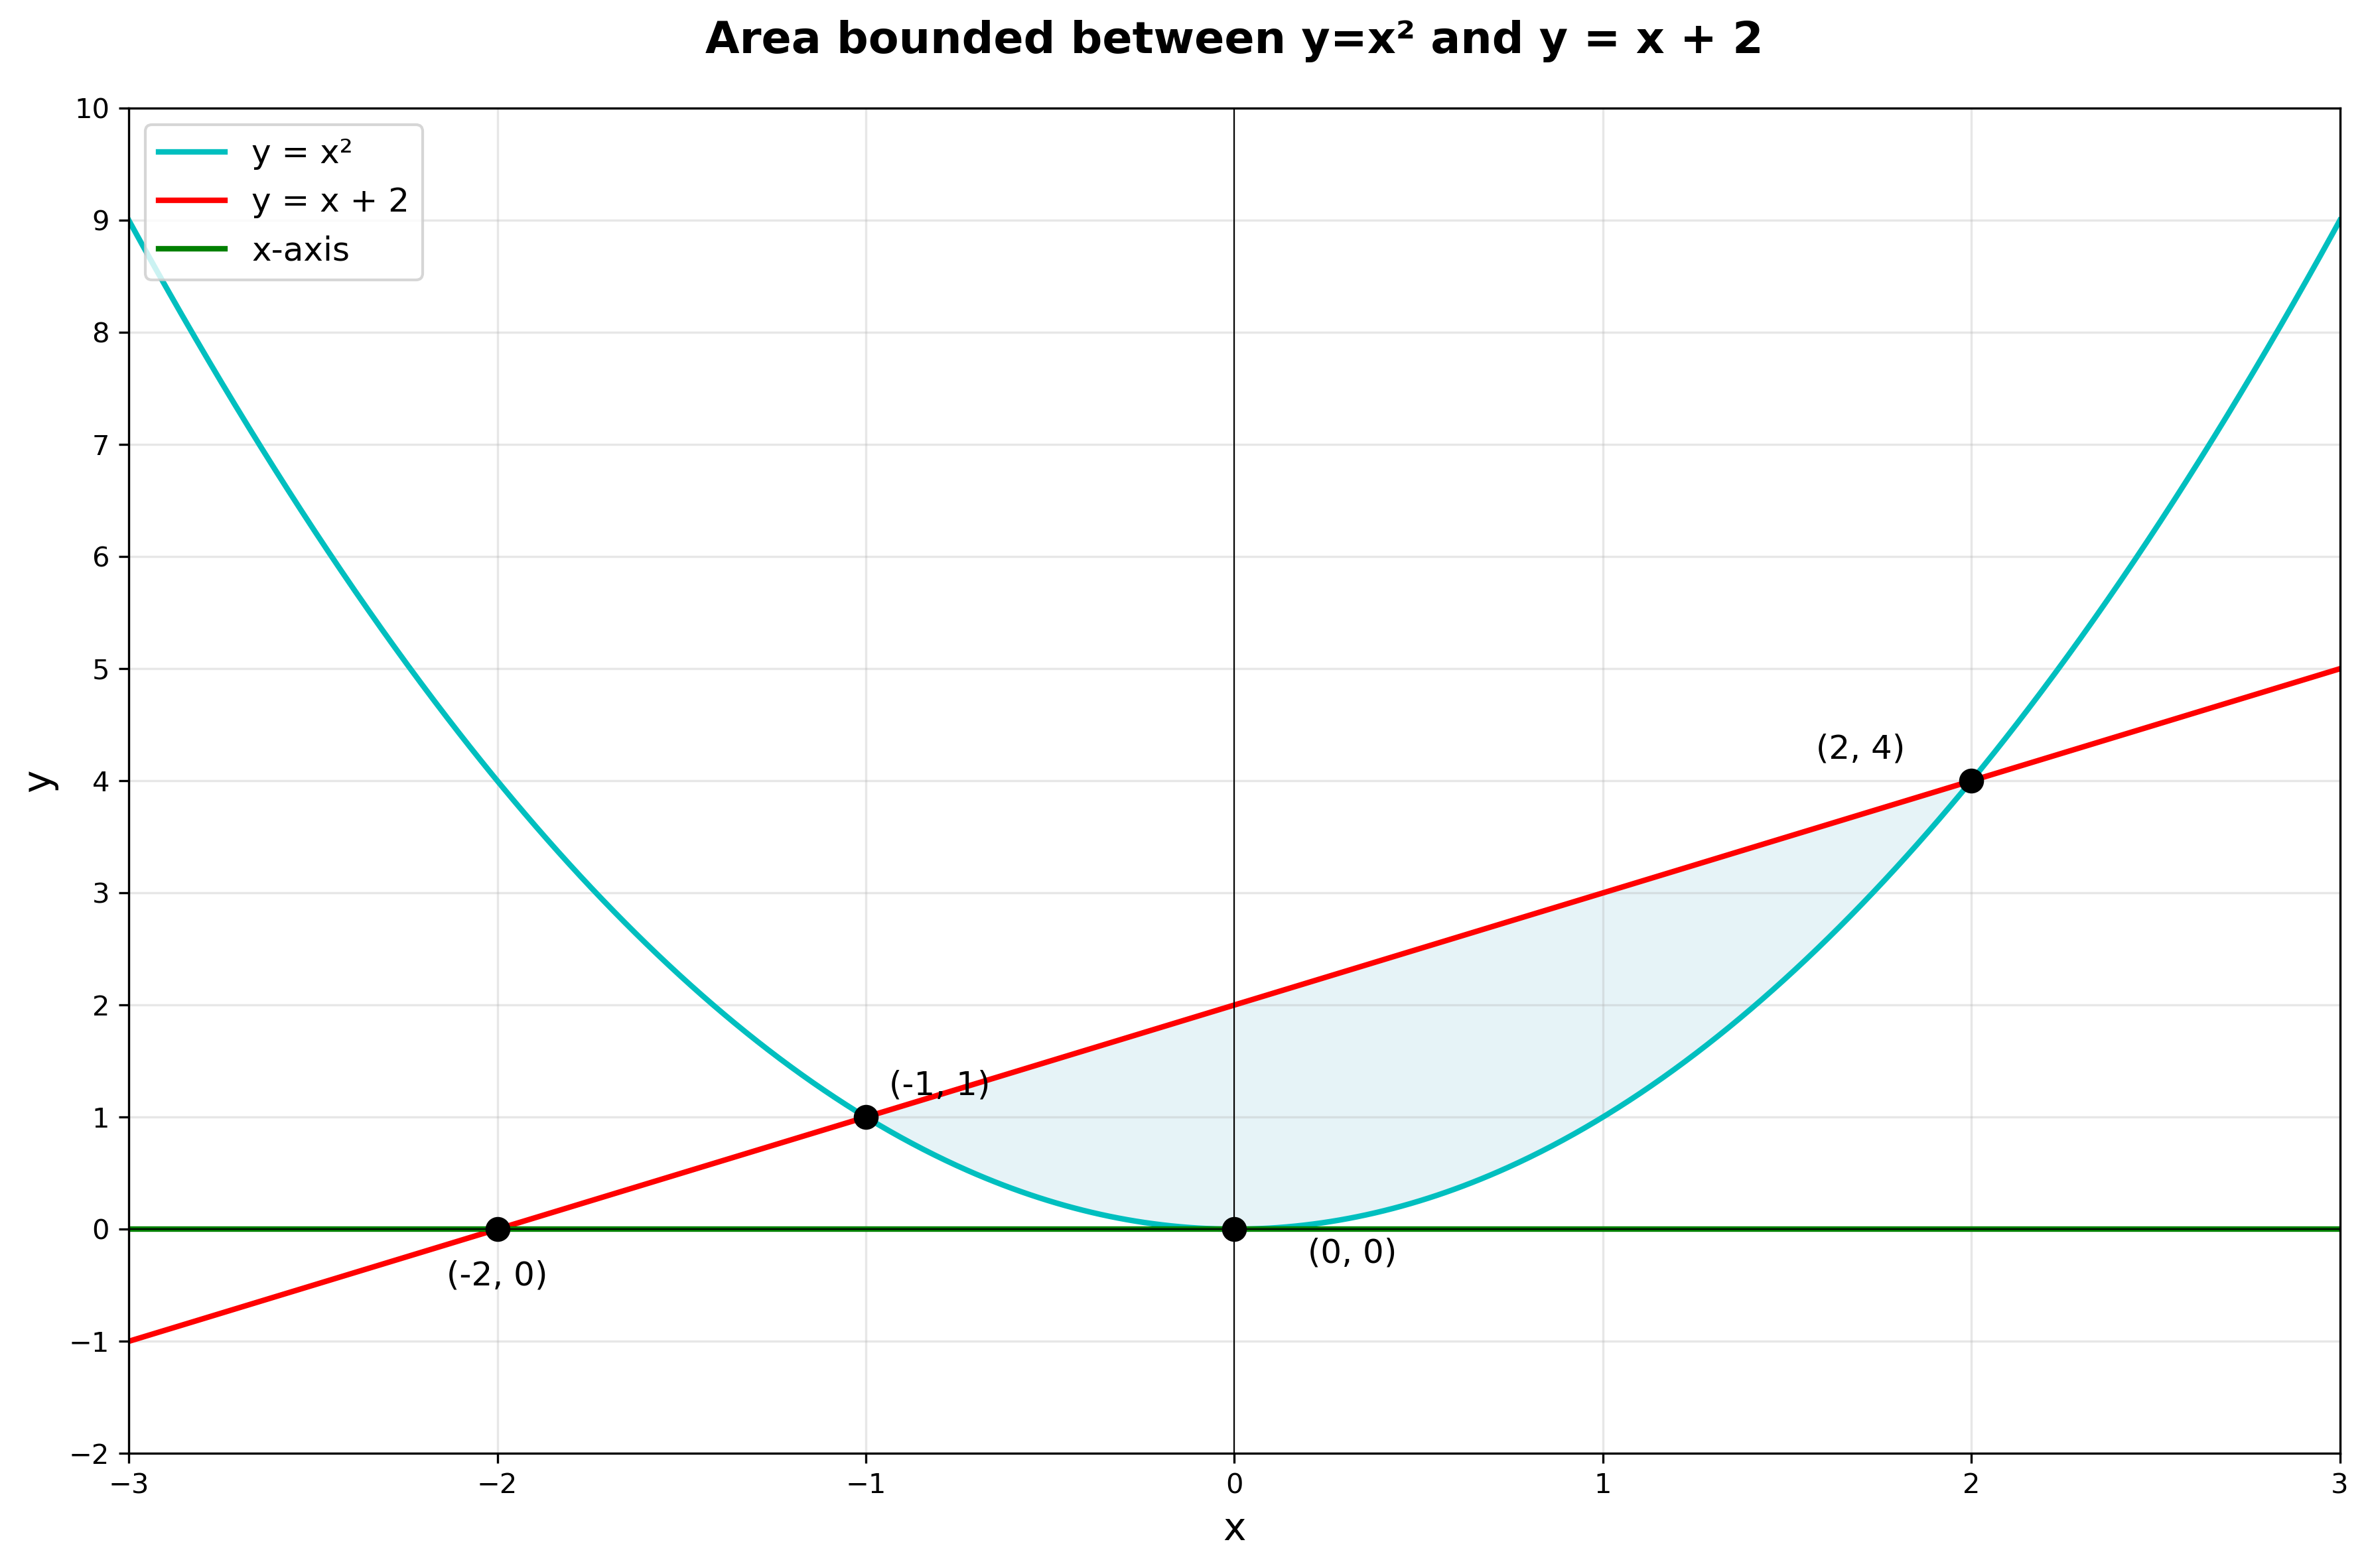
\includegraphics[width=\columnwidth]{figs/fig1.png}
    \caption{Intersection of Conic and Line}
    \label{fig:figs/fig1.png}
\end{figure}

\end{document}  
